\chapter{Characterization of Grouping Problems} \label{chap:grouping_problems} 

    In this chapter, we explore the characterization of grouping problems, focusing on their definitions, common types, and recent developments. We begin by defining how grouping problems are approached in industry. This concept is then related to graph theory, where vertices represent objects and edges represent connections, providing a theoretical framework for understanding grouping problems \cite{newman2018networks}.
    
    We then delve into common types of grouping problems, including explicit matching, implicit matching, one-to-one matching, one-to-many matching, many-to-many matching, user-item matching, and others \cite{gusfield1989stable, demange1986multi}. Each type presents unique challenges and applications in various industries.
    
    Finally, we discuss recent developments in the field of grouping problems, including advanced algorithms for solving matching problems efficiently and applications in diverse fields such as quantum computing \cite{quantum_matching}, artificial inteligence \cite{gnn_graph_matching, cross_modal_matching}, and Humanitarian and Resource Allocation \cite{humanitarian_routing}. By examining these developments, we aim to provide a comprehensive overview of the current state of grouping problems and their significance in various domains \cite{ieee_survey}.
    
\section{How to Define an Industry Matching (Grouping) Problem}

    In industry, matching problems are problems where the objective is to match some elements, usually the optimizing an objective function.
    %%
    Importantly, in industry, the concept of matching problems is often not bounded to the graph theory definition of matching problems.
    %%
    For that reason, we refer to grouping problems as a larger set of problems, which includes not only graph theory's matching problems, but also other problems that can be represented as a graph, where the objective is to group objects based on some criteria.

    When faced with a set of objects, such as job openings and candidates, the objective is to group these objects, assigning candidates to jobs in this context, where each group generates a set of statistics, and this statistics are used to optimize an objective function. This concept is well-established in the field of operations research and combinatorial optimization \cite{manlove2013algorithmics}.

    \subsection{Job Assignment} \label{subsec:job_assignment}
        One of the most well-known examples of a grouping problem is job assignment. The objective is to match job positions with candidates who possess the necessary skills, experience, and qualifications. The process involves considering the specific requirements of each position and the attributes of the candidates, aiming to maximize overall efficiency or satisfaction. This type of problem has been widely studied, particularly in the context of labor markets and automated recruitment systems \cite{roth1990two}.

    \subsection{Resource Allocation} \label{subsec:resource_allocation}
        Resource allocation problems involve distributing limited resources—such as rooms, equipment, or funds—among competing tasks or projects. The challenge lies in ensuring that the allocation maximizes efficiency while meeting constraints, such as availability and demand. These problems are critical in industries like healthcare, manufacturing, and project management, where effective resource distribution directly impacts outcomes \cite{schrijver2003combinatorial}.
    
    \subsection{Network Routing} \label{subsec:network_routing}
        In network routing problems, the goal is to determine the optimal way to route data, goods, or resources through a network. This involves minimizing costs, delays, or energy consumption while ensuring that demands are met across the network. Such problems are particularly relevant in logistics, telecommunications, and supply chain management, where optimizing flow is essential for performance \cite{ahuja1993network}.
    
    \subsection{Stable Matching} \label{subsec:stable_matching}
        Stable matching problems focus on creating pairings where no two entities would prefer being matched with each other over their current assignments.
        %
        The stable marriage problem is a classic example, where the objective is to create stable pairs based on mutual preferences. Applications of stable matching range from college admissions processes to organ donation programs, where stability and fairness are crucial \cite{gusfield1989stable, demange1986multi}.
        %
        These problems are fundamental in various industries and have been extensively studied \cite{manlove2013algorithmics}.


    \subsection{Industrial Terminology compared to Graph Theory}
    
   In the context of graph theory, vertices may represent objects, and edges represent the connections or relationships between these objects \cite{west2001introduction, diestel2017graph}. 
    This basic terminology is crucial when translating industrial problems into graph models.

    Edges often contain statistics that can represent preferences, costs, capacities, and other characteristics.
    For example, in the stable marriage problem  (see Subsection \ref{subsec:stable_matching}), edges' statistics represent preferences between pairs \cite{gale1962college}.
    In the Hungarian algorithm for the assignment problem  (see Subsection \ref{subsec:resource_allocation}), edges represent costs associated with assignments \cite{kuhn1955hungarian}. 
    In network flow problems (see Subsection \ref{subsec:network_routing}), edges represent capacities that limit the amount of flow through the network \cite{ford1956maximal}.
    
    For industry applications, any graph cover problems are often collectively referred to as matching problems \cite{larman2004applying, fowler2003patterns}. However, to avoid confusion, in the context of this work, we will use the terms ``grouping'' and ``matching"" interchangeably.

    For instance, in a logistics network, vertices could represent warehouses and stores, while edges represent possible delivery routes. 
    Finding an optimal set of routes that minimizes cost can be modeled as a grouping problem.
    %
    Using this terminology allows us to frame complex industrial problems in a structured way, making it easier to apply graph-theoretical algorithms and techniques to find optimal solutions.
    
    
    \section{Usual Matching Problems}
        
        In this section, grouping problems will be referred to as "matching" problems, as this is how they are often called in the industry. The categorization of problems into subcategories, based on the classification provided by the survey \cite{ieee_survey}, reveals several common grouping problem structures, such as explicit and implicit matching. Table \ref{tbl:summarisation_applications_matching} shows a detailed relation of problems, characteristics, and applications. Other characteristics that can be applied to all problems include online/offline (dynamism), scalability, heterogeneity, noise tolerance, and privacy requirements \cite{ieee_survey}.
        
        \begin{table}
    \centering
    \scalebox{0.64}{
        \begin{tabular}{|c|c|c|c|c|}
            \hline
            \textbf{Category}                   & \textbf{Sub-category}                     & \textbf{Algorithms}                     & \textbf{References}                                                                                                                           & \textbf{Applications}                                                                                                           \\ \hline
            \multirow{4}{*}{Explicit Matching}  & One-to-one Matching                       & -                                       & \cite{gale1962college,roth1992two,becker1973theory,bergstrom1993courtship}                                                                                                        & marriage market                                                                                                                 \\ \cline{2-5} 
                                                & \multirow{2}{*}{Many-to-one 
                                                Matching}     & \multirow{2}{*}{-}                      & \cite{bergstrom1993courtship,gale1962college,roth1992two,rosen1981economics,roth1984stability}                                                                                              & job matching                                                                                                                    \\ \cline{4-5} 
                                                &                                           &                                         & \cite{kremer1993ring,gabaix2008ceo,tervio2008ceo}                                                                                                                 & pay matching                                                                                                                    \\ \cline{2-5} 
                                                & Many-to-many Matching                     & Optimization algorithms                 & \cite{gabaix2008ceo,bergstrom1993courtship,roth1992two,becker1973theory}                                                                                                         & \begin{tabular}[c]{@{}c@{}}cognitive radio networks; \\ D2D communications\end{tabular}                                         \\ \hline
            \multirow{11}{*}{Implicit Matching} & \multirow{3}{*}{Retrieval Matching}       & Traditional matching algorithms         & \cite{ramos2003using,salton1988term,becker1973theory,dumais2004latent,hofmann1999probabilistic,bergstrom1993courtship}                                                                                    & \multirow{3}{*}{\begin{tabular}[c]{@{}c@{}}machine translation;\\ expertise matching; \\ question-answer matching\end{tabular}} \\ \cline{3-4}
                                                &                                           & Representation-based algorithms         & \cite{bengio2009learning,bengio2009learning,he2017neural,che2019stable}                                                                                                       &                                                                                                                                 \\ \cline{3-4}
                                                &                                           & Interaction-based algorithms            & \begin{tabular}[c]{@{}c@{}}\cite{dumais2004latent,bengio2009learning,che2019stable,che2019stable,becker1973theory}, \\\cite{gabaix2008ceo,che2019stable,dumais2004latent,roth1992two,becker1973theory}\end{tabular} &                                                                                                                                 \\ \cline{2-5} 
                                                & \multirow{3}{*}{User-item Matching}       & Basic algorithms                        & \cite{su2009survey,che2019stable}                                                                                                                            & \multirow{3}{*}{recommendation systems}                                                                                         \\ \cline{3-4}
                                                &                                           & Representation-based algorithms         & \cite{pang2016text,dumais2004latent,koren2015advances,dumais2004latent,roth1992two}                                                                                              &                                                                                                                                 \\ \cline{3-4}
                                                &                                           & Matching function-based algorithms      & \cite{blei2003latent,bengio2009learning,he2017neuralfm,gabaix2008ceo}                                                                                                       &                                                                                                                                 \\ \cline{2-5} 
                                                & \multirow{3}{*}{Entity-relation Matching} & Factorization-based algorithms          & \cite{dumais2004latent,bay2008surf,gabaix2008ceo,gabaix2008ceo}
                                                & \multirow{3}{*}{\begin{tabular}[c]{@{}c@{}}recommendation systems;\\ knowledge fusion; \\ information retrieval\end{tabular}}   \\ \cline{3-4}
                                                &                                           & Neural network-based algorithms         &  \cite{rosen1981economics,blei2003latent,becker1973theory,roth1992two}                                                                                                      &                                                                                                                                 \\ \cline{3-4}
                                                &                                           & Translational distance-based algorithms &  \cite{rosen1981economics,roth1992two,dumais2004latent,bergstrom1993courtship,roth1992two}                                                                                             &                                                                                                                                 \\ \cline{2-5} 
                                                & \multirow{2}{*}{Image Matching}           & Area-based algorithms                   & \cite{blei2003latent,gruen1985adaptive,dumais2004latent,dumais2004latent,yang2018image}                                                                                              & \multirow{2}{*}{\begin{tabular}[c]{@{}c@{}}robot vision; \\ object recognition;\\ medical image diagnosis\end{tabular}}         \\ \cline{3-4}
                                                &                                           & Feature-based algorithms                & \begin{tabular}[c]{@{}c@{}}\cite{blei2003latent,lowe2004distinctive,gabaix2008ceo,becker1973theory,rosen1981economics}, \\ \cite{rosen1981economics,roth1992two,blei2003latent,roth1992two,roth1992two}\end{tabular} &                                                                                                                                 \\ \hline
        \end{tabular}
    }
\caption{Summarisation of Matching Algorithms and Applications According to \cite{ieee_survey}.}
    \label{tbl:summarisation_applications_matching}
\end{table}

        
        Matching problems can be broadly divided into two main categories: explicit and implicit.
        
        \subsection{Explicit Matching}
            Explicit matching problems involve objects that have preferences about whom they prefer to group with \cite{ieee_survey, manlove2013algorithmics}. These can be further categorized into:
            
            \begin{itemize}
                \item \textbf{One-to-one}: also known as bipartite matching, common in job assignment where each job is assigned to a single candidate and vice versa \cite{kuhn1955hungarian}.
                \item \textbf{Many-to-one}: found in scenarios like college admissions, where multiple students can be assigned to a single college \cite{gale1962college}.
                \item \textbf{Many-to-many}: occurs in contexts such as organ donation, where multiple donors can provide organs to multiple recipients \cite{roth2004kidney}.
            \end{itemize}
        
        \subsection{Implicit Matching}
            Implicit matching focuses on calculating the 'score' of the grouping without explicit preferences, optimizing based on a grouping function \cite{ieee_survey}. Examples include:
            
            \begin{itemize}
                \item \textbf{Retrieval Matching}: in information retrieval, it involves users inputting queries that express their needs and obtaining the desired information from a search engine's database \cite{manning2008introduction}.
                \item \textbf{User-item Matching}: in recommender systems, it helps users obtain items of interest accurately \cite{ricci2011introduction}.
                \item \textbf{Entity-relation Matching}: it involves the use of knowledge graphs in applications such as semantic parsing, information extraction, link prediction, recommender systems, and question answering \cite{ji2021survey}.
                \item \textbf{Image Matching}: it compares different images to identify similarities or correspondences, used in fields like computer vision and pattern recognition \cite{szeliski2010computer}.
            \end{itemize}

        

   \section{Recent Developments}

    The field of matching problems is constantly evolving, with ongoing research introducing new problems, solutions, and algorithmic approaches to address the complexity and diversity of these challenges in industry. In this section, we outline a preliminary review aimed at identifying the latest developments in matching problems, focusing on advancements made since 2021.

    To capture the most recent and relevant studies, we conducted an initial search in Google Scholar on \textbf{January 19, 2025}, using the following search string:

    \begin{quote}
    (TITLE-ABS-KEY("pairing") OR TITLE-ABS-KEY("matching") OR TITLE-ABS-KEY("grouping")) AND (TITLE-ABS-KEY("solver") OR TITLE-ABS-KEY("algorithm")) AND TITLE-ABS-KEY("graph") AND PUBYEAR AFTER 2021
    \end{quote}

    The query was executed using a command-line Python tool named \texttt{scholar.py}\footnote{\texttt{scholar.py} is an open-source command-line utility that allows querying Google Scholar and retrieving citation metadata programmatically. See: \url{https://github.com/ckreibich/scholar.py}}, which automates the retrieval of publication metadata such as titles, abstracts, and citation counts. This approach enabled a structured and replicable filtering process.

    The review process involved applying inclusion criteria to select studies that contribute to the development of matching algorithms, whether through incremental improvements, novel problem types, algorithmic frameworks, or solvers that expand the applicability of matching techniques in industry.

    After collecting the top 100 studies by number of citations, they were filtered by language, retaining only those in English. Then, based on titles and abstracts, works unrelated to matching were removed, including six that focused on diverse clustering problems. Although clustering problems may be addressed by the general solution proposed in Chapter~\ref{chap:design}, they are out of scope and suggested as future work in Chapter~\ref{chap:conclusion}. Figure~\ref{fig:bib} illustrates the selection process, showing the number of studies removed and retained at each stage. Furthermore, we analyze the most prominent topics that emerged from the remaining studies.

    \begin{figure}[!ht] \label{gig:bib}
\centering

\tikzstyle{process} = [rectangle, minimum width=1.5cm, minimum height=6.5cm, text centered, draw=black, fill=white, text width=1.75cm, font=\small]
\tikzstyle{mid_process} = [rectangle, minimum width=1cm, minimum height=1cm, text centered, draw=black, fill=white, text width=1.75cm, font=\small]
\tikzstyle{arrow} = [thick,->,>=stealth]

\scalebox{0.7}{%
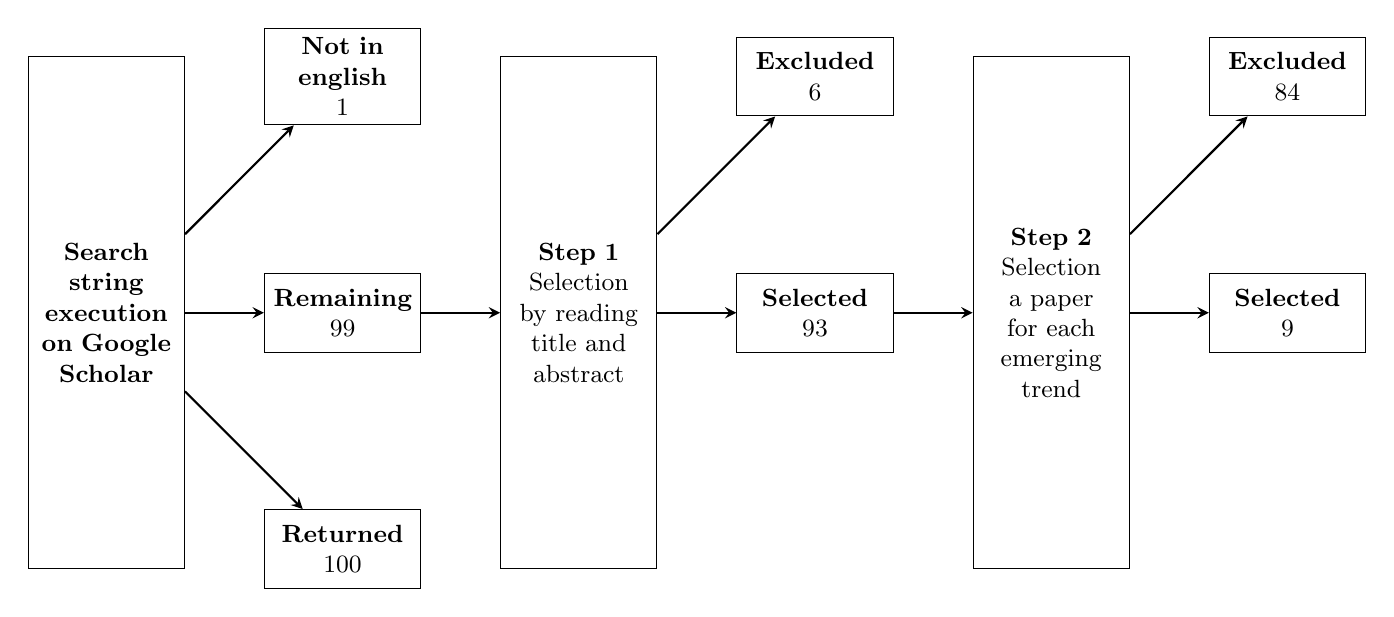
\begin{tikzpicture}[node distance=3cm, auto]

    % Nodes
    \node (start) [process] {\textbf{Search string execution on Google Scholar}};
    \node (remaining) [mid_process, right of=start] {\textbf{Remaining} \\ 99};
    \node (repeat) [mid_process, above of=remaining] {\textbf{Not in english} \\ 1};
    \node (returned) [mid_process, below of=remaining] {\textbf{Returned} \\ 100};
    
    \node (step1) [process, right of=remaining] {\textbf{Step 1} \\ Selection by reading \\ title and abstract};
    \node (included1) [mid_process, right of=step1] {\textbf{Selected} \\ 93};
    \node (excluded1) [mid_process, above of=included1] {\textbf{Excluded} \\ 6};


    \node (step2) [process, right of=included1] {\textbf{Step 2} \\ Selection a paper for each \\ emerging trend};
    \node (included2) [mid_process, right of=step2] {\textbf{Selected} \\ 9};
    \node (excluded2) [mid_process, above of=included2] {\textbf{Excluded} \\ 84};

    % Arrows
    \draw [arrow] (start) -- (remaining);
    \draw [arrow] (start) -- (repeat);
    \draw [arrow] (start) -- (returned);
    
    \draw [arrow] (remaining) -- (step1);
    \draw [arrow] (step1) -- (excluded1);
    \draw [arrow] (step1) -- (included1);

    
    \draw [arrow] (included1) -- (step2);
    \draw [arrow] (step2) -- (excluded2);
    \draw [arrow] (step2) -- (included2);
    

\end{tikzpicture}
}

\caption{Selection Process of the Articles.}
\label{fig:bib}
\end{figure}
    
    \subsection{Overview of Recent Existing Approaches}
    Table \ref{tbl:old_types} presents a summary of the selected studies in step 1, categorizing them based on their focus and contributions to the field of matching. Each study is classified according to the definitions of Implicit Matching by \cite{ieee_survey}. Additionally, we detail the common subjects treated by the new publications.

    

    \begin{table}[ht]
\centering
\begin{tabular}{|c|c|}
\hline
\textbf{Implicit Matching Category} & \textbf{Total} \\
\hline
Retrieval Matching & 16 \\
User-item Matching & 10 \\
Image Matching & 33 \\
Entity-relation Matching & 34 \\
\hline
\end{tabular}
\caption{Total of Works after step 1 by Implicit Matching Category.}
\label{tbl:old_types}
\end{table}

    
    This review aims to demonstrate the breadth of recent developments in matching, highlighting both the versatility of applications and the growing need for centralized tools that simplify the implementation and adaptation of matching solutions across various industrial contexts.

    \subsection{Emerging Trends in Graph Matching Algorithms}
        Here we overview the 9 selected studies about emerging trends.
        \begin{enumerate}
            \item \textbf{Quantum Computing}
            \begin{itemize}
                \item \textbf{Trend:} Quantum computing is starting to impact optimization and matching algorithms. Some works suggest that quantum algorithms are being explored for graph-based problems, particularly in sparse data and matching contexts \cite{quantum_matching}.
                \item \textbf{Context:} Quantum algorithms may offer exponential speedup over classical methods in certain areas, and combining quantum techniques with combinatorial optimization is a growing field.
            \end{itemize}
            
            \item \textbf{AI and Deep Learning in Graph Matching}
            \begin{itemize}
                \item \textbf{Trend:} Many studies focus on graph neural networks (GNNs) and deep learning in graph matching \cite{gnn_graph_matching, cross_modal_matching}.
                \item \textbf{Context:} AI, particularly deep learning, is being applied to improve the accuracy and efficiency of graph matching, especially in image recognition, NLP, and multi-modal data integration.
            \end{itemize}
        
            \item \textbf{Video and Image Recognition}
            \begin{itemize}
                \item \textbf{Trend:} Recognition algorithms using graph matching are becoming more common, especially in computer vision \cite{image_keypoint_matching}.
                \item \textbf{Context:} This is closely related to AI, where graph-based methods are used for tasks like multi-object tracking and 3D object detection.
            \end{itemize}
        
            \item \textbf{Combinatorial Algorithms and Optimization}
            \begin{itemize}
                \item \textbf{Trend:} Classical combinatorial algorithms remain an important area of research \cite{faster_bipartite_matching}.
                \item \textbf{Context:} These algorithms are central in problems like scheduling, resource allocation, and network flow.
            \end{itemize}
        
            \item \textbf{Networks and Multi-Agent Systems}
            \begin{itemize}
                \item \textbf{Trend:} Network theory and multi-agent systems use graph matching for optimization \cite{network_matching, privacy_graph_matching}.
                \item \textbf{Context:} These topics focus on applications in wireless communication, sensor networks, and privacy-preserving computation.
            \end{itemize}
        
            \item \textbf{Cross-modal and Multi-modal Matching}
            \begin{itemize}
                \item \textbf{Trend:} Matching across different types of data (e.g., text and images) is an emerging trend in AI and cross-modal retrieval \cite{cross_modal_matching}.
                \item \textbf{Context:} These algorithms are applicable in industries like e-commerce, digital media, and autonomous systems.
            \end{itemize}
        
            \item \textbf{Humanitarian and Resource Allocation Applications}
            \begin{itemize}
                \item \textbf{Trend:} Graph matching and optimization algorithms are used in resource allocation and humanitarian problems \cite{humanitarian_routing}.
                \item \textbf{Context:} This trend focuses on real-world applications like disaster management and healthcare.
            \end{itemize}
        
            \item \textbf{Graph Matching for Knowledge Graphs and Semantic Systems}
            \begin{itemize}
                \item \textbf{Trend:} Knowledge graphs and semantic matching are gaining attention in AI reasoning and data integration \cite{knowledge_graph_matching}.
                \item \textbf{Context:} These methods are key in NLP, semantic web technologies, and AI-driven data systems.
            \end{itemize}
        
            \item \textbf{Privacy and Security in Graph Matching}
            \begin{itemize}
                \item \textbf{Trend:} Privacy-preserving graph matching is a significant concern, particularly for sensitive data \cite{privacy_graph_matching}.
                \item \textbf{Context:} These methods are relevant in domains like healthcare, finance, and social networks.
            \end{itemize}
        \end{enumerate}
        